\section{Návrh strategické hry}

Zpracováno na základě: \cite{navrh_lenses} \cite{navrh_rules} \cite{navrh_level}.

V této kapitole rozeberu postup návrhu jednoduché strategické hry hrané na náhodně vygenerované mapě.

Návrh strategické hry vyžaduje systematický přístup k definování jejích klíčových prvků. Aby byla hra hratelná, vyvážená a pokud možno i zábavná, je zapotřebí systematicky rozebrat a promyslet návrh všech částí hry. 

Základní představa, se kterou jsem začínal před samotným systematickým návrhem, byla taková, že hra bude 2D tahová strategie se správou surovin. Hráči budou ovládat a vylepšovat své jednotky, spravovat zdroje a budovat infrastrukturu, přičemž se budou snažit dosáhnout vítězství nad soupeřem. Herní svět je reprezentován dlaždicovou mapou, typ terénu na dlaždici ovlivňuje pohyb jednotek, možnosti výstavby a dostupnost zdrojů.

Pro návrh hry využívám metodologii z knihy \textit{The Art of Game Design: A Book of Lenses} od Jesseho Schella, která strukturuje herní design do několika klíčových kategorií:

\begin{itemize}
    \item Prostor -- Jak je herní svět uspořádán a jak se v něm hráči pohybují.
    \item Objekty, atributy a stavy -- Jaké herní entity existují, jaké mají vlastnosti a jaké stavy mohou při hře nastat.
    \item Akce hráče -- Jaké interakce může hráč provádět a jak ovlivňují hru.
    \item Pravidla hry -- Jaká jsou omezení a podmínky vítězství.
    \item Dovednost a náhoda -- Jaký je poměr mezi strategickým rozhodováním a prvky náhody.
\end{itemize}

Tento rámec poskytuje ucelený pohled na návrh hry a pomáhá zajistit, aby všechny prvky dohromady tvořily soudržný a dobře vyvážený celek.

Ve zbytku kapitoly rozeberu podrobněji právě tyto herní prvky a konkretizuji herní návrh.

%-------------------------------------------------------------------------
\subsection{Prostor}

Každá hra obsahuje nějaký herní prostor, ve kterém se celá hra odehrává. Ten obecně vymezuje herní lokace a určuje, jak jsou mezi sebou propojeny. Z pohledu herních mechanik je považován prostor za matematickou konstrukci, tedy je potřeba odfiltrovat veškeré vizuální prvky a zaměřit se pouze na abstraktní uspořádání prostoru.

Kniha \textit{The Art of Game Design: A Book of Lenses} rozděluje herní prostory podle několika parametrů:

\begin{itemize}
    \item Diskrétnost vs. kontinuita -- Prostor může být buď diskrétní, nebo kontinuální. Diskrétní prostor je tvořen pevně stanovenými, oddělenými místy. Kontinuální prostor umožňuje pohyb v plynulém, nekonečném rozsahu.
    \item Počet dimenzí -- Každý herní prostor má určitý počet dimenzí, které definují jeho rozsah a strukturu. Prostor může být jednorozměrný, dvourozměrný nebo dokonce třírozměrný.
    \item Ohraničenost a propojení oblastí -- Prostor může být uzavřený, s pevně definovanými hranicemi, nebo otevřený, umožňující pohyb hráče nebo herních prvků mimo hranice.
\end{itemize}

Příklad hry hrané na diskrétním dvoudimenzionálním poli je "piškvorky" (v rámci příkladu předpokládám herní plochu $3\times3$), kde herní plocha je rozdělena na devět oddělených políček. Herní deska je zobrazena jako souvislý prostor, ale z hlediska herních mechanik bereme v potaz pouze těchto devět specifických míst, která můžeme znázornit jako uzly v síti. Tedy dokud je jednoznačně rozeznatelné, do kterého políčka zapadá, jsou si mechanicky ekvivalentní, jak je naznačeno na obrázku \vref{sudoku}.

\begin{figure}
  \centering      % vycentrovat
  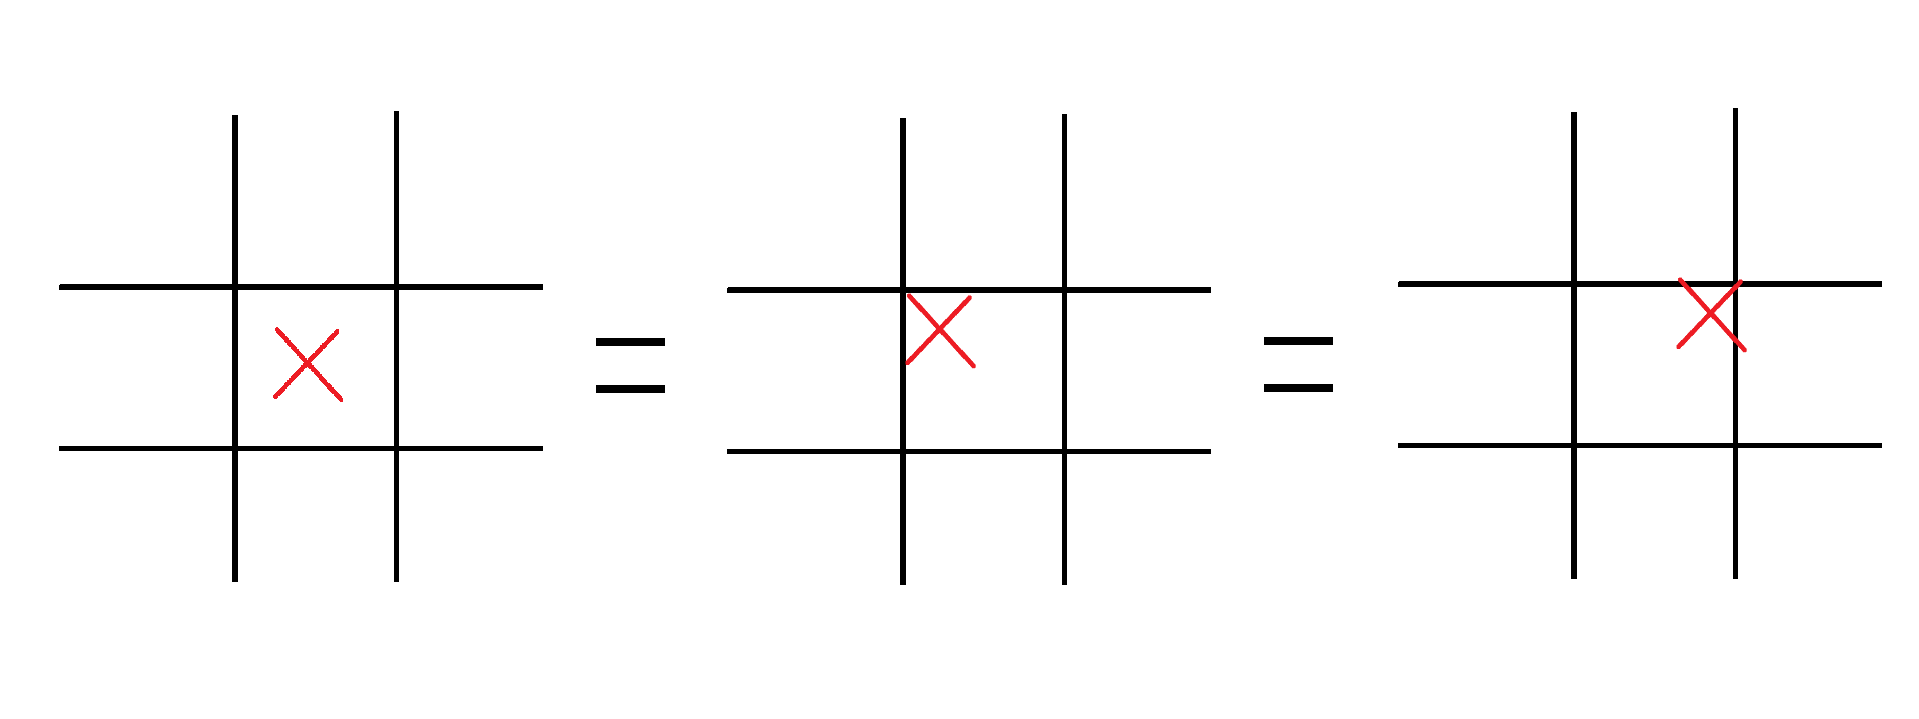
\includegraphics[scale=0.3]{obr/sudoku.png} % soubor + měřítko (scale)
  \caption{Ekvivalence různých značení sudoku.} % popis obrázku
  \label{sudoku} % definice odkazu na obrázek (pro \ref{})
\end{figure}

Hra monopoly je pak příklad jednodimenzionální hry. I když je herní deska vizuálně uspořádána do tvaru čtverce, když se odstraní grafické prvky, můžeme vidět, že hra umožňuje pohyb po jediné řadě políček, propojených v cyklické smyčce. V tomto případě se každé políčko na desce chová jako bod nulové dimenze, ačkoliv vizuálně vypadají některé čtverce odlišně, jejich funkce se neliší.

Herní prostor může také zahrnovat „prostory v prostorech“, což se často vyskytuje v počítačových hrách. Například může existovat venkovní prostor (kontinuální, dvourozměrný), ale hráč může narazit na ikony, které představují města nebo jeskyně. Tyto ikony přecházejí do zcela oddělených prostorů, které s venkovním prostorem nejsou přímo propojené, což je příkladem prostorového uspořádání, které je více založeno na mentálních modelech hráčů než na geografické realitě.

\subsubsection{Návrh herního prostoru}

Jak jsem již zmínil, navrhovaná hra bude 2D tahová strategie, tedy herní prostor bude dvoudimenzionální a diskrétní, složený ze čtvercových políček propojených po horizontální a vertikální ploše. To bude mít zásadní vliv na pohyb jednotek po mapě a tedy i veškerá strategická rozhodnutí hráčů.

Diskrétnost herního prostoru usnadňuje měření vzdáleností, po které se jednotky mohou po desce pohybovat, a také omezuje rozložení budov na jednu budovu na políčko. To samé platí pro jednotky, což umožňuje strategické tahy, jako blokování pohybu jednotek nepřítele.

Ve hře nebudou žádné podprostory ani oblasti, které by hráči mohli navštívit jako separátní oblasti. Všechny interakce probíhají na jednom herním poli, přičemž všechny herní mechaniky se soustředí na strategické využití této plochy.

Z hlediska návrhu a pozdější implementace tedy herní prostor uvažuji jako dvourozměrné diskrétní pole, kde každé "políčko" představuje bod s nulovou dimenzí. Tento pohled by měl zjednodušit návrh pravidel a interakcí mezi hráči a prostředím, což umožňuje efektivnější rozvoj herních taktik.

%-------------------------------------------------------------------------
\subsection{Objekty, atributy a stavy}


V herním prostoru se pak nacházejí objekty, se kterými hráči v průběhu celé hry manipulují nebo s nimi interagují pomocí jiných objektů. Může se jednat například o herní figurky, postavy, karty, nebo samotné herní prostředí. Objekty lze chápat jako „podstatná jména“ herních mechanik. 

Každý objekt má nějaké atributy, které popisují jeho vlastnosti. Atributy lze chápat jako "přídavná jména". Například auta v závodní hře mohou mít atributy jako \textit{maximální rychlost} a \textit{aktuální rychlost}. 

Každý herní objekt má \textbf{stav}, který určuje jeho vlastnosti a chování ve hře. Stav objektu se skládá z jeho atributů, což jsou jednotlivé charakteristiky objektu. Například figurka v šachu má atribut „mód pohybu“, který může nabývat stavů jako „volně se pohybující“, „v šachu“ a „matovaná“. V Monopoly má každý pozemek atribut „počet domů“, jehož stav se může měnit mezi 0 až 4 domy nebo hotel.

Atributy mohou být statické nebo dynamické:

\begin{itemize} \item Statické atributy – Nemění se v průběhu hry. Například barva figurky v dámě nebo maximální rychlost auta.
\item Dynamické atributy – Mohou se měnit v závislosti na akcích hráčů či mechanikách hry. Například aktuální rychlost auta se mění podle řízení hráče, životy jednotky klesají při útoku. \end{itemize}

Každý herní objekt tak může mít kombinaci statických a dynamických atributů. Například v šachu má figurka statický atribut „barva“, ale dynamický atribut „pozice na šachovnici“, který se mění během hry.

Je důležité si uvědomit, že objekty ve hře často interagují mezi sebou. Například, jednotka může útočit na jinou jednotku, budova může produkovat suroviny, nebo terénní prvek může ovlivňovat pohyb jednotek. Tyto interakce by měly být navrženy tak, aby dávaly smysl a byly pro hráče srozumitelné.

Stav objektu není nutně viditelný celý – některé atributy mohou být skryté nebo viditelné jen pro určité hráče.

Důležitou součástí herního návrhu tedy je rozhodnout, kdo má přístup k jakým informacím. Pro jednoduchost rozlišíme informace na \textit{veřejné} \textit{částečně skryté} nebo \textit{zcela skryté}. 

\begin{itemize}
    \item Veřejné informace -- Všechny atributy a jejich stavy jsou viditelné pro všechny hráče. Například v šachu oba hráči vidí všechna pole a figurky na hrací desce, takže jediným tajemstvím je přemýšlení soupeře.
    \item Částečně skryté informace -- Někteří hráči znají určitou informaci, ale jiní ne. Například ve hře poker někteří hráči viděli kartu, zatímco jiní ne.
    \item Zcela skryté informace -- Existují atributy, které zná pouze samotná hra. Například v počítačových hrách mohou být některé části světa před hráčem skryté, dokud je neodhalí.
\end{itemize}

Rozhodnutí o tom, kdo má přístup k jakým informacím, zásadně ovlivňuje herní strategii a atmosféru. Hry jako poker jsou postavené na utajení a odhadu soupeřových karet, zatímco v šachu mají hráči k dispozici informace o stavu celé herní plochy, a jedinou neznámou je strategie protivníka.

\subsubsection{Návrh herních objektů}

V této části se podle probraných principů pokusím nastínit jednotlivé objekty a definovat atributy těchto objektů.

Ve hře se nachází několik typů objektů, se kterými hráči mohou manipulovat nebo s nimi interagovat. Základním objektem ve hře jsou \textbf{políčka} ze kterých je složené herní pole a určují podmínky pro pohyb jednotek a stavbu budov. \textbf{Budovy}, produkují suroviny, případně poskytují další služby a plní jiné strategické funkce. Jako poslední jsou \textbf{jednotky} což jsou pohyblivé objekty ovládané hráčem, které hráč využívá k různým činnostem, jako je boj, nebo těžba surovin. Každý z těchto objektů má své specifické atributy a stavy, které určují jejich vlastnosti a možnosti ve hře.

Co se informací týče, nakonec jsem se rozhodl, že hra nebude mít skryté informace, tedy hráči od začátku uvidí celý herní prostor a pohyby protivníka.


\paragraph{Políčka}
Políčka představují základní stavební jednotku mapy, na níž se odehrává hra. Každé políčko má několik atributů, popisujících jeho vlastnosti a interakce s ostatními objekty. Tyto atributy jsou:
\begin{itemize}
    \item Statické:
    \begin{itemize}
        \item \textbf{Pozice na mapě} -- Souřadnice určující umístění políčka v herním prostoru.
        \item \textbf{Název} -- Název terénu.
        \item \textbf{Zpomalení} -- Určité typy terénů mohou snižovat pohybovou rychlost jednotek. 
        \item \textbf{Bonusová obrana} -- Některé terény mohou zvyšovat obranu jednotek na daném políčku.
        \item \textbf{Získatelné suroviny} -- Typ surovin které je možné na políčku získat.
    \end{itemize}
    \item Dynamické:
    \begin{itemize}
        \item \textbf{Obsazenost jednotka} -- Na políčku se může nacházet pouze jedna jednotka, tento atribut tedy bude bránit vstupu jiné jednotky na políčko.
    \item \textbf{Obsazenost budova} -- Na políčku může stát pouze jedna budova.
    \end{itemize}
%    \item \textbf{Možné zdroje} – některá políčka obsahují suroviny jako dřevo, kámen nebo jídlo. 
%    \item \textbf{Zpomalení} – některé terény zpomalují pohyb jednotek.
\end{itemize}

Terén není jen grafický prvek, ale významně ovlivňuje hru. Správná volba umístění jednotek může znamenat rozdíl mezi vítězstvím a porážkou – například jednotka stojící na horách má lepší obranu, zatímco husté lesy mohou zpomalit postup nepřátel. Navíc různé druhy terénu určují, jaké budovy lze postavit a jaké suroviny lze těžit.



\paragraph{Budovy}
Budovy jsou struktury, které hráči staví na mapě za účelem generování zdrojů nebo poskytování jiných výhod. Každá budova má následující atributy:
\begin{itemize}
    \item Statické:
    \begin{itemize}
        \item \textbf{Pozice na mapě} -- Pozice budovy na herní mapě.
        \item \textbf{Název} -- Označení budovy.
        \item \textbf{Vlastník} -- Určuje hráče, kterému budova patří. Změna vlastníků během hry nebude možná, pouze zničení nepřátelských budov.
        \item \textbf{Typ terénu} -- Omezení, na kterých typech políček lze budovu postavit.
        \item \textbf{Produkce za kolo} – množství surovin, které budova generuje za kolo.
        \item \textbf{Životy max} -- Maximální počet životů budovy.
        \item \textbf{Obrana} -- O kolik se zredukuje poškození způsobené útokem.
        \item \textbf{Cena} -- Množství surovin potřebných pro stavbu budovy.
        \item \textbf{Bonusová obrana} -- Budova může zvyšovat obranu jednotek nacházejících se na stejném políčku.
        \item \textbf{Speciální funkce} -- Budova může umožňovat provádění speciálních akcí jako generování nebo vylepšování jednotek.
    \end{itemize}
    \item Dynamické:
    \begin{itemize}
        \item \textbf{Životy} -- Aktuální počet životů budovy, pokud klesne na nulu budova je zničena.
    \end{itemize}
\end{itemize}
Budovy kromě generování surovin poskytují hráči jiné strategické možnosti jako vylepšování jednotek, zvyšování obrany vlastních jednotek nebo blokování postupu nepřítele.

\paragraph{Jednotky}
Jednotky jsou pohyblivé objekty na mapě, které hráči ovládají a skrze které primárně interagují s herními mechanismy. Každá jednotka má své atributy, které určují její vlastnosti a schopnosti:
\begin{itemize}
    \item Statické:
    \begin{itemize}
        \item \textbf{Název} -- Název typu jednotky.
        \item \textbf{Pozice na mapě} -- Kde na herním poli se jednotka nachází.
        \item \textbf{Vlastník} – hráč, kterému jednotka patří.
        \item \textbf{Cena} -- Množství surovin potřebné pro vytvoření jednotky.
        \item \textbf{Cena za kolo} -- Náklady na udržování jednotky. Množství surovin které jednotka spotřebuje každé kolo.
        \item \textbf{Životy max} -- Maximální počet životů jednotky.
         \item \textbf{Základní obrana} -- Základní obrana jednotky. Redukuje poškození způsobené nepřátelským útokem.
        \item \textbf{Útok} -- Síla útoku. Určuje o kolik se sníží životy nepřátelské jednotky při útoku. Poškození je redukované obranou. 
        \item \textbf{Dosah} -- Vzdálenost, na kterou může jednotka útočit.
        \item \textbf{Základní rychlost} – Maximální počet políček, která může jednotka urazit za kolo.
    \end{itemize}
    \item Dynamické:
    \begin{itemize}
        \item \textbf{Životy} -- Aktuální počet životů jednotky, pokud klesne na nulu jednotka zmizí.
        \item \textbf{Obrana} -- Funkční obrana jednotky, po modifikaci prostředím (Typem terénu nebo budovou.).
        \item \textbf{Rychlost} -- Skutečný počet políček přes který se jednotka může v daném tahu pohybovat, po modifikaci terénem.
        \item \textbf{Zaměstnaná} -- Indikuje, zda jednotka vykonala akci v tomto tahu.
        \item \textbf{V pohybu} -- Indikuje zda se jednotka v tahu pohybovala.
        \item \textbf{Zkušenosti} -- Jednotka může být vylepšena v konkrétní budově po dosažení určitého počtu zkušeností, které získává prováděním akcí odpovídajících jejímu typu (válečníci získávají zkušenosti bojem, pracovníci těžbou surovin nebo opravami budov).
    \end{itemize}
\end{itemize}

Jednotky představují hlavní způsob, jak hráč ovlivňuje dění na mapě. Každá jednotka má specifickou roli – některé slouží k boji, jiné k těžbě surovin nebo stavbě budov. Postupem času mohou získávat zkušenosti a vylepšovat své schopnosti, což přidává další vrstvu strategického rozhodování. Kromě toho jednotky také každé kolo spotřebovávají množství surovin, tedy hráč musí zvážit, zda si může dovolit postavit velkou armádu slabých jednotek.


%-------------------------------------------------------------------------
\subsection{Akce hráče}

Akce jsou jedním ze základních stavebních kamenů herní mechaniky. Lze je chápat jako "slovesa“ hry, jelikož definují, jak může hráč interagovat s herním světem. Rozdělujeme je do dvou hlavních kategorií:

\begin{itemize}
    \item \textbf{Operační akce} jsou základní činnosti, které může hráč přímo vykonat, například pohyb jednotky nebo útok.
    \item \textbf{Výsledné akce} vycházejí z kombinace operačních akcí. Tyto emergentní akce často nejsou přímo definovány pravidly, ale vznikají přirozeně během hry a přispívají k její hloubce.
\end{itemize}

\textbf{Operační akce} jsou základní mechanismy, které hráč využívá pro interakci s herními mechanismy. V některých hrách je množství těchto akcí omezené, což vede k menší variabilitě herního stylu, zatímco v jiných hrách mají hráči širokou škálu možností, což umožňuje kreativní přístupy. Například ve hře dáma má hráč k dispozici tři základní operační akce:
\begin{itemize}
    \item Posun kamene vpřed.
    \item Přeskok soupeřova kamene.
    \item Pohyb zpět v případě dosažení úrovně krále.
\end{itemize}

\textbf{Výsledné akce} vznikají kombinací operačních akcí a přispívají ke strategické hloubce hry. Zatímco operační akce jsou pevně dané pravidly, výsledné akce se objevují jako důsledek interakcí mezi hráčem, herním prostředím a protivníky. Ve hře dáma mohou být výslednými akcemi například:
\begin{itemize}
    \item Ochrana kamene -- umístění jiného kamene za něj, aby zabránil zajetí.
    \item Vynucení tahu soupeře -- postavení figurky tak, že soupeř musí provést nevýhodný tah.
    \item Obětování kamene -- nabídnutí figurky soupeři s cílem získat lepší pozici na hrací ploše.
\end{itemize}
Výsledné akce přidávají hře hloubku a umožňují emergentní chování hráče. Čím větší je poměr výsledných akcí vůči operačním akcím, tím více hra podporuje kreativitu hráče.

\subsubsection{Návrh herních akcí}

V této části rozeberu obecné operační akce, které bude hráč moci ve hře provádět, a následně zmíním vzniklé výsledné akce.

V rámci tahového systému může hráč během svého tahu každou jednotkou provést pohyb a jednu další akci. Některé akce mohou proběhnout pouze pokud jsou splněny určité podmínky, například pozice jednotky v určité budově. Vzhledem k tahovému systému a interakci mezi jednotkami a terénem mohou vznikat nové strategie, které nelze vždy předvídat.

\paragraph{Operační akce} jsou základní činnosti, které může hráč vykonávat, primárně interakcí se svými jednotkami.
\begin{itemize}
    \item Pohyb -- Jednotka se pohne o počet polí odpovídající jejímu typu a terénu.
    \item Útok -- Jednotka zaútočí na nepřátelskou jednotku v dosahu, způsobí poškození (\textit{poškození = útok - obrana}) a pokud nepřítel přežije, provede protiútok.
    \item Těžba surovin -- Pracovní jednotka získá určité množství surovin na základě toho na jakém terénu těžba proběhne.
    \item Práce -- Pracovní jednotka v budově může získávat větší množství surovin, v budově která normálně generuje suroviny pasivně.
    \item Stavba budovy -- Budovatelská jednotka postaví novou budovu na vhodném políčku.
    \item Oprava budovy -- Pracovní nebo budovatelská jednotka obnoví část života poškozené budovy.
    \item Vylepšení jednotky -- Pokud jednotka splní požadavky (např. bojové zkušenosti, existenci potřebné budovy, ...), může být vylepšena na silnější variantu.
\end{itemize}

\paragraph{Výsledné akce} vznikají kombinací operačních akcí a strategického uvažování hráče.
\begin{itemize}
    \item Obrana klíčových bodů -- Hráč umístí jednotky tak, aby blokovaly přístup k důležitým budovám nebo oblastem.
    \item Napadání zásobování -- Cílený útok na pracovníky nebo budovy snižující zdroje nepřítele.
    \item Taktický ústup -- Ústup jednotek do bezpečnější oblasti, například k opravám nebo pod ochranu budov.
    \item Obklíčení -- Koordinovaný útok více jednotek k eliminaci klíčových nepřátel.
    \item Zdržovací taktika -- Hráč strategicky obětuje jednotky nebo využívá terén, aby zpomalil postup nepřítele.
    \item Ofenzivní opevnění -- Hráč staví budovy poblíž nepřátelské základy jako obranné pozice.
\end{itemize}


%-------------------------------------------------------------------------
\subsection{Pravidla hry}

Pravidla určují, jak se hra hraje, jaké akce může hráč provádět a jaké jsou jeho cíle. Bez jasně definovaných pravidel není možné vytvořit funkční a férové herní prostředí.

Špatně strukturovaná pravidla mohou vést k nevyváženosti, nechtěným eksploačním mechanikám nebo dokonce ke ztrátě zábavnosti. Správně nastavená pravidla zároveň hráče motivují k objevování efektivních strategií k dosažení vítězství.


Pravidla jsou soubor omezení a možností, které definují, jak hráči interagují s herním světem. V každé hře existují různé typy pravidel, která ovlivňují hratelnost:

\begin{itemize}
    \item Akce hráčů -- Co mohou hráči během hry dělat?
    \item Stav hry -- Jak se hra mění v průběhu času?
    \item Cíle hry -- Kdy hra končí a kdo vyhrává?
\end{itemize}
Tato pravidla společně vytvářejí herní mechaniky, které určují dynamiku hry a poskytují hráčům výzvy k řešení.

David Parlett, britský herní teoretik, rozdělil pravidla do několika kategorií:

\begin{itemize}
    \item Operační pravidla -- Popisují základní akce hráčů, například „hráč se může pohnout o $n$ políček“.
    \item Základní pravidla -- Definují matematický model hry, určují, jak se hra vyvíjí na základě akcí hráčů.
    \item Chování hráčů -- Implicitní pravidla "fair play" a sportovního chování.
    \item Psaná pravidla -- Formálně dokumentovaná pravidla hry.
    \item Zákony -- Další pravidla, která mohou být zavedena například pro turnajovou hru.
    \item Oficiální pravidla -- Spojují psaná pravidla a zákony do jednoho uceleného souboru.
    \item Doporučená pravidla -- Tipy a strategie pro efektivní hraní.
    \item Domácí pravidla -- Úpravy pravidel hráči pro přizpůsobení hry jejich preferencím.
\end{itemize}

Herní pravidla mohou být ovlivněna herním režimem, který může do hry přidávat komplexitu přidáním nebo odebráním pravidel. Případně úpravou podmínek vítězství.

Nejdůležitějším pravidlem jsou cílové podmínky. Každá hra musí mít jasně definovaný cíl, který hráče motivuje a určuje, kdy hra končí. Dobrý cíl by měl splňovat:

\begin{itemize}
    \item Konkrétnost -- Je jasné, co musí hráči udělat.
    \item Dosažitelnost -- Hráči mají reálnou možnost dosáhnout cíle.
    \item Odměňující charakter -- Splnění cíle přináší uspokojení.
\end{itemize}

\subsubsection{Návrh pravidel}

V této části shrnu dosavadní návrh do konkrétních pravidel. Pravidla definují podmínky vítězství, možné akce hráčů a interakce mezi herními objekty.

Primárním cílem hry je poražení protivníka, což je dosaženo zničením všech jeho jednotek a budov. Hra tedy končí, když zůstane pouze jeden hráč.

Sekundární cíle si hráč stanovuje sám, ale zahrnují:

\begin{itemize}
    \item Efektivní správa ekonomiky -- těžba surovin a stavba podpůrných budov.
    \item Budování armády -- rekrutování a vylepšování jednotek.
    \item Dobývání strategických bodů -- kontrola území s cennými zdroji nebo taktickými výhodami.
\end{itemize}

\paragraph{Objekty} Hra obsahuje tři typy herních objektů:

\begin{itemize}
    \item Jednotky
    \begin{itemize}
        \item Bojové -- primárně slouží k útoku a obraně (např. válečník).
        \item Stavební -- mohou stavět nové budovy, opravovat poškozené budovy a těžit suroviny.
    \end{itemize}
    
    \item Budovy
    \begin{itemize}
        \item Ekonomické -- pasivně produkují zdroje (např. důl).
        \item Obranné -- poskytují ochranu a strategickou kontrolu území.
        \item Vývojové -- umožňují vylepšovat jednotky na vyšší úroveň.
    \end{itemize}
    
    \item Terén
    \begin{itemize}
        \item Ovlivňuje pohyb a bojové vlastnosti jednotek. (Např. hory zpomalují pohyb, lesy poskytují krytí, voda je nepřekročitelná.)
    \end{itemize}
    
\end{itemize}

\paragraph{Akce} V každém tahu může hráč provést s každou svou jednotkou jeden pohyb a jednu akci s tím, že některé akce vyžadují specifické podmínky, například vylepšení vyžadují určité budovy nebo sběr surovin má různý efekt podle terénu. Akce zahrnují:

\begin{itemize}
    \item Pohyb jednotek
    \begin{itemize}
        \item Každá jednotka se pohybuje pouze vertikálně a horizontálně, diagonální pohyb není možný.
        \item Terén ovlivňuje pohyb jednotek (např. hory snižují jejich pohybovou vzdálenost).
    \end{itemize}
    
    \item Útok
    \begin{itemize}
        \item Hráč vybere útočníka v dosahu.
        \item Útok je vyhodnocen podle atributů jednotek (útok vs. obrana).
        \item Pokud obránce přežije, provede protiútok.
    \end{itemize}
    
    \item Výstavba a interakce s objekty
    \begin{itemize}
        \item Stavební jednotky mohou budovat budovy na určitých místech.
        \item Pracovní jednotky mohou těžit suroviny, případně opravovat budovy
    \end{itemize}
\end{itemize}

\paragraph{Vynucování pravidel} Pravidla jsou automaticky vynucována herním systémem: Hráč může provádět pouze akce, které jsou v dané situaci povolené (např. jednotky nemohou cestovat přes políčka s vodou). Výsledky bojů jsou deterministické, hra tedy automaticky udělí způsobené poškození, případně zruší jednotku, pokud její životy klesnou na nulu. Hra automaticky končí, jakmile některý hráč přijde o všechny jednotky a budovy a tedy nemůže provést žádnou další akci.

%-------------------------------------------------------------------------
\subsection{Skill and Chance (Dovednost a náhoda)}
\begin{itemize}
    \item Jaký vliv má dovednost hráče na výsledek hry:
    \begin{itemize}
        \item Strategické plánování.
        \item Správné rozhodování a reakce na situace.
    \end{itemize}
    \item Jaký vliv má náhoda:
    \begin{itemize}
        \item Procedurálně generovaná mapa jako faktor variabilních podmínek.
    \end{itemize}
    \item Vyvážení mezi dovedností a náhodou.
\end{itemize}


%-------------------------------------------------------------------------
\subsection{Shrnutí}
\begin{itemize}
    \item Shrnutí hlavních bodů návrhu.
    \item Vztah návrhu k procedurálnímu generování map.
\end{itemize}
